\section{Pre-treatment of Cu-foils: Polishing}

\paragraph{Experiment realization}The first attempt to etch the Cu-foil was performed with the $5\%_{vol}$ EG, $25\%_{vol}\,H_2O$ filled up with phosphoric acid. The etching was performed in a \SI{200}{\ml} beaker, filled with \SI{150}{\ml} etching solution. The setup is as depicted in \autoref{fig:etching-setup}. The potential was adjusted to be \SI{1.2}{\V} after some minutes. The current through the solution changes and is typically highest when the etching process started. 

After some minutes the foils reflectivity changes. The foils surface - shiny before etching - becomes hazy. After some more time the foils reflectivity improves again. When no visual change to the surface is observed the etching process is interrupted. 

The time inside the etching solution depends on the handling (like shaking the beaker or moving the foil in the solution - but was usually $\geq \SI{2}{\hour}$.
%\footnote{Since the perfect voltage/current to perform polishing varies in time a automated etching process has been developed \cite{palmieri_besides_2001}}

One has to be careful if reproducible results are needed. During the etching process (as more and more copper settles on the counter electrode), the current and therefore the etching rate decreases continuously. When the beaker is moved, some of the debris on the electrode changes (the electrode's) surrounding and the etching rate (limiting current) increases again. 
Front- and backside of the foil are suspect to different etching processes. The back side is generally more flat, the side facing the counter-electrode always shows some additional protrusions.

\paragraph{After etching treatment}
The foil is taken out and cleaned from remaining etchants with purified water first and isopropanol afterwards. Foils are be stored in isopropanol to avoid oxidation.\footnote{To further improve the quality of the foil, one can follow the documented recipe for annealing the foil in a $H_2$ atmosphere (\SI{10}{sscm}, \SI{1000}{\celsius}, 30min)\cite{kim_synthesis_2012} to increase the copper grain size and further smoothen the surface. We decided to further prepare the foils within the UHV chamber and skipped this step.}

\paragraph{AFM}
\label{sec:foil-AFM}
\begin{figure}[] \centering
	\subfigure[Copper foil before etching.]{
		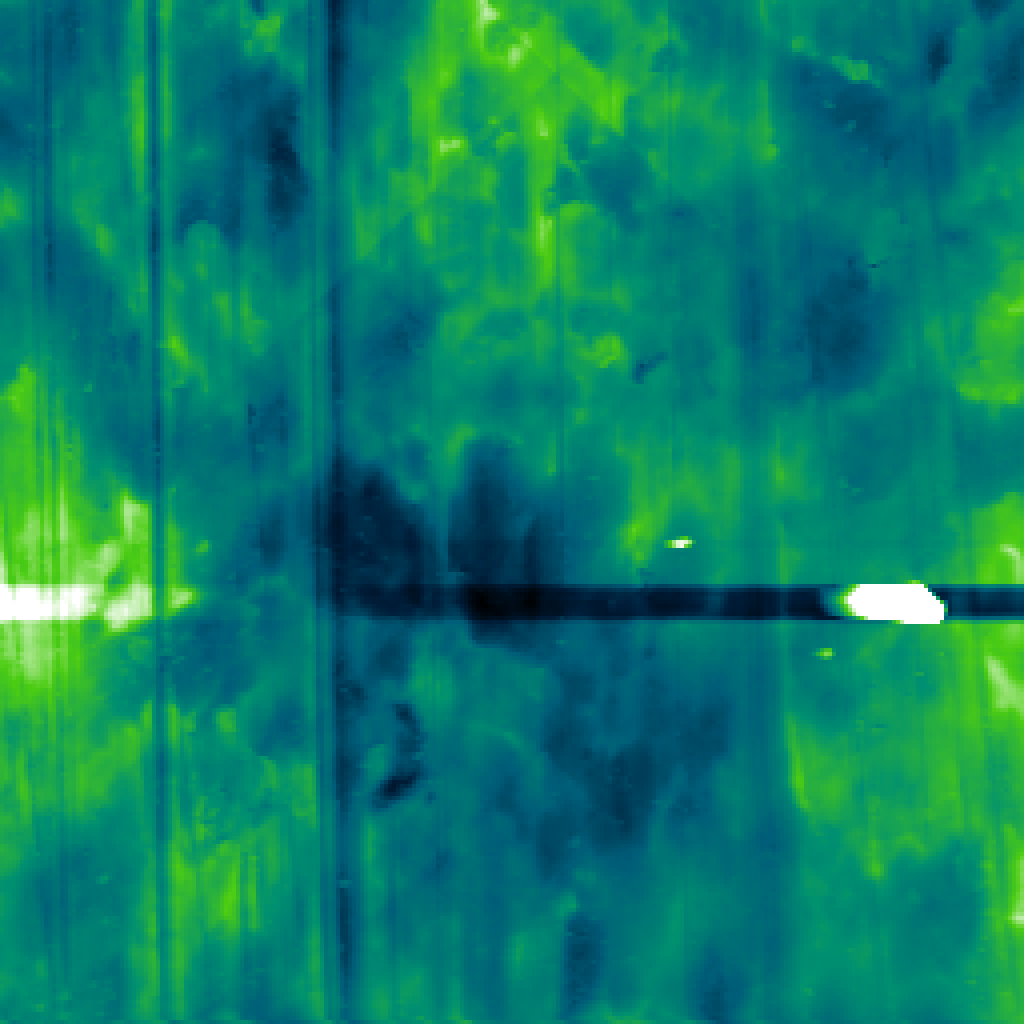
\includegraphics[width=0.35\textwidth]{./images/as_bought0000}
		\label{fig:foil-bought-afm}
	} \quad
	\subfigure[Copper foil after etching]{
		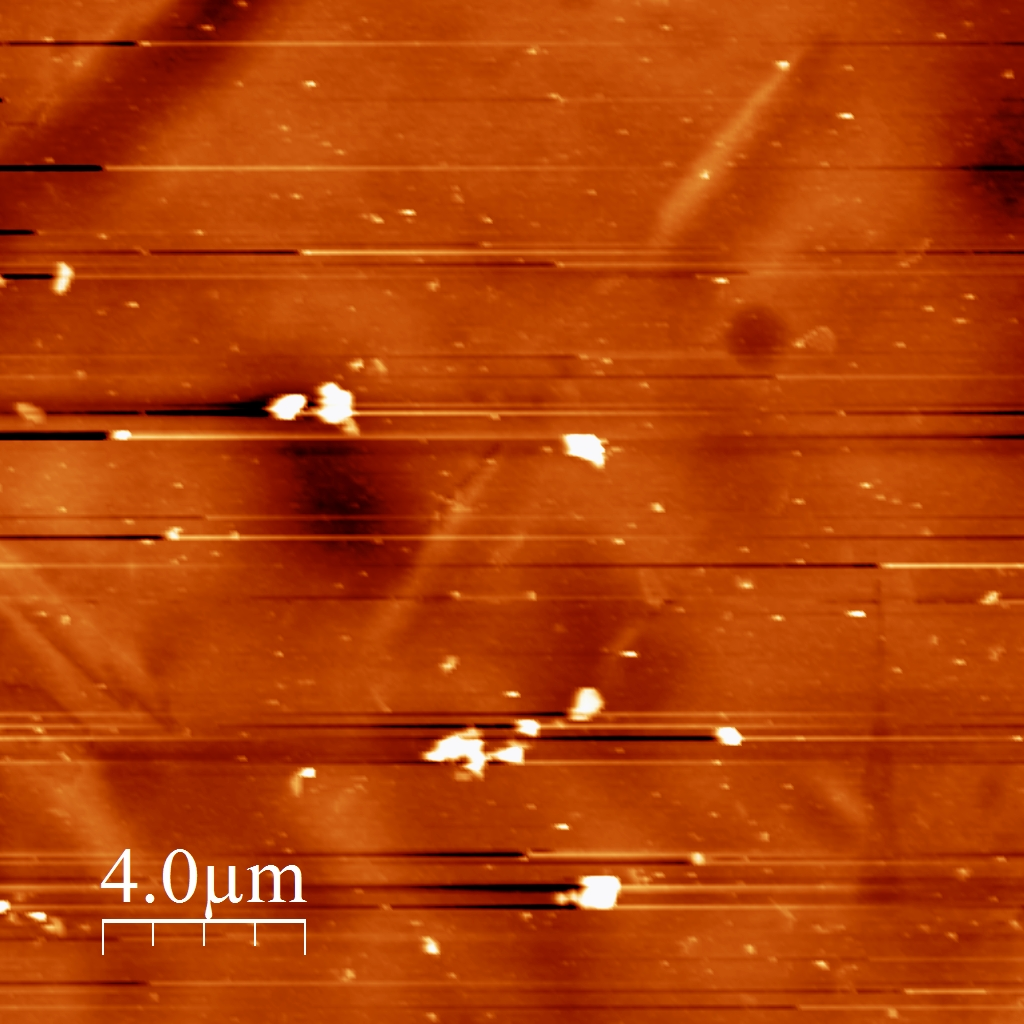
\includegraphics[width=0.35\textwidth]{./images/polished0000}
		\label{fig:foil-polished-afm}
	}
	\subfigure[Height profiles of the two samples.]{
		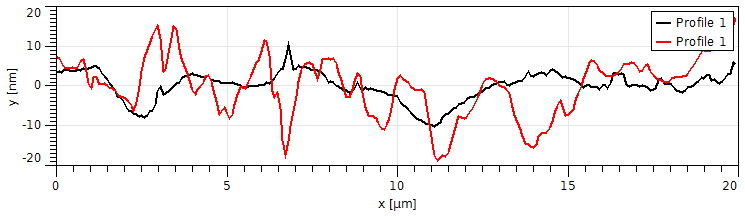
\includegraphics[width=0.7\textwidth]{./images/as_bought-polished_0000-profiles}
		\label{fig:foil-profiles}
	}
	\caption{AFM topography image of copper foil as bought from Alfa Aesar \subref{fig:foil-bought-afm} before and \subref{fig:foil-polished-afm} after etching. \subref{fig:foil-profiles} Height profile averaging the lower 10 lines of \subref{fig:foil-bought-afm} and \subref{fig:foil-polished-afm}. Roughness along the line profiles decreases after etching ($Rq_{before}=\SI{7.3}{\nano \meter} \rightarrow Rq_{after}=\SI{3.6}{\nano \meter}$). Color scale for both AFM images \SI{100}{\nano \meter} \textcolor{red}{\textbf{Image width: \SI{20}{\micro \meter}IMAGING PARAMETERS!}}}
	\label{fig:foil-afm-as-bought}
\end{figure}

Figure \ref{fig:foil-bought-afm} shows the striations that stem from the production process (from top to buttom).
%\begin{figure}[] \centering
%	\subfigure[RMS $\approx$\SI{9}{\nm} in the left image, contrast \SI{100}{\nm}]{
%	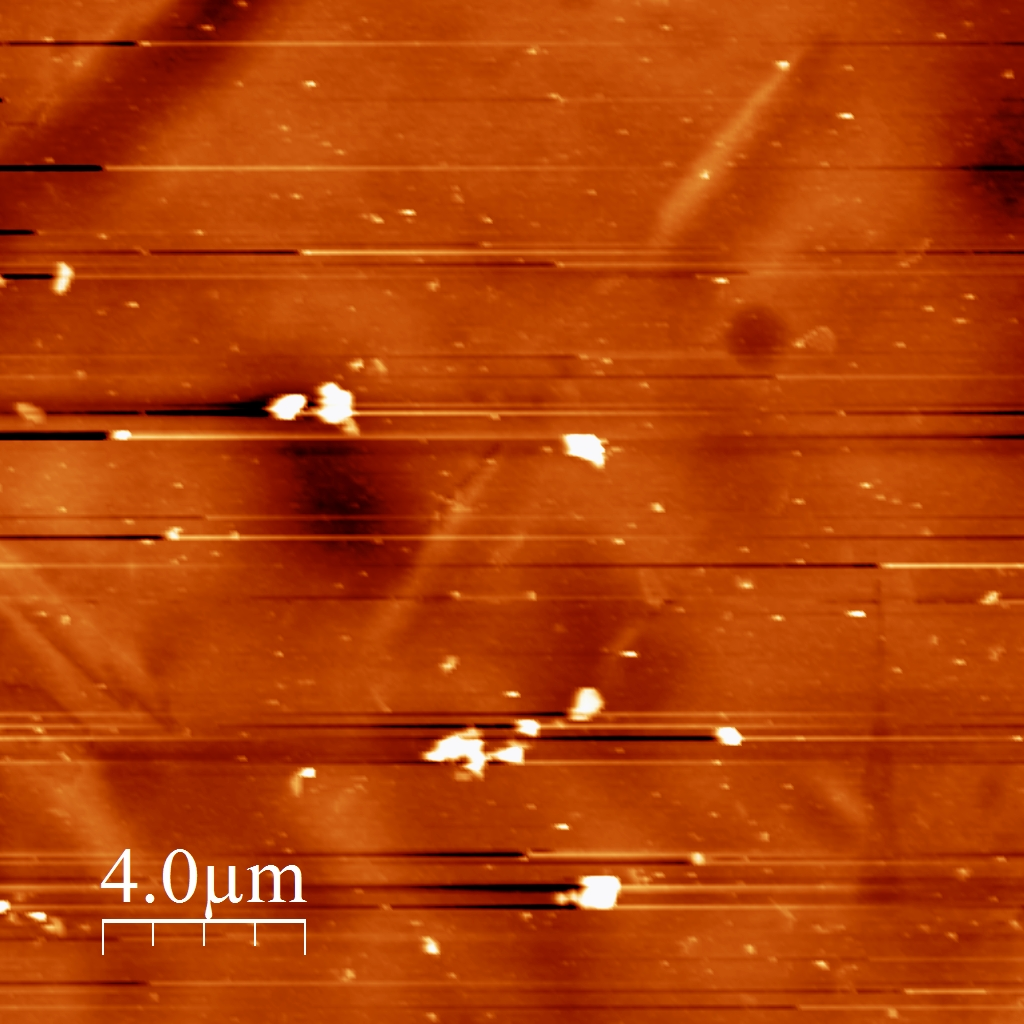
\includegraphics[width=0.4\textwidth]{./images/polished0000.jpg}
%}
%	\subfigure[RMS $\approx$\SI{3}{\nm} in the right image, contrast \SI{70}{\nm}]{
%	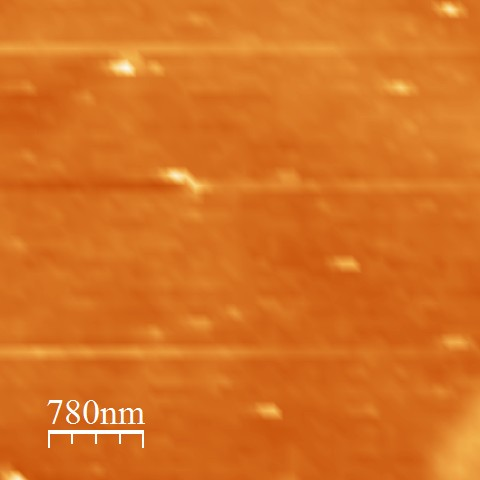
\includegraphics[width=0.4\textwidth]{./images/polished0001.jpg}
%}
%	\caption{AFM image of a copper foil polished 5h (according to table \ref{tab:used-etching-solution}), \textcolor{red}{\textbf{IMAGING PARAMETERS!}}}
%	\label{fig:foil-afm-polished}
%\end{figure}

After etching ($U=1.2V$,I=\SIrange{120}{250}{\mA}) for \SI{5}{\hour} in a solution (shown in table \ref{tab:used-etching-solution}) the striations have gone and the RMS value decreased by \SI{50}{\percent} and an increase in foil quality is obvious even with bare eyes. Figure \ref{fig:foil-afm-as-bought} and \ref{fig:foil-afm-polished} show AFM images in the same size and contrast - before and after etching.
The circular hole is an effect of bubbles in the etching process where the bubble affects the rate of etching. The over all structure changes from a heterogenous sample height to a flat height contribution with only a little amount of defects. Those are sufficiently seperated in space to exhibit flat regions where the h-BN may grow unperturbated.
%
%\paragraph{SEM}
%\label{sec:foil-SEM}
%Invented in the 1930's by Manfred von Ardenne\cite{ardenne_elektronen-rastermikroskop_1938}, Scanning electron microscopy (SEM)\index{SEM} is another versatile tool for the experimentalist. In contrast to (LT-)STM and AFM, SEM is capable of imaging huge areas of the sample within a very short time, which allows for a vast overview as well as good statistics. Magnifications reach up to 500k and above, illustrating even features in the order of \SI{1}{\nano \meter}.

As the name already discloses, SEM scans the surface with electrons. Their interaction with the material are diverse and some of them are explained in the following. While all effects are present in every measurement, not every microscope features detectors for all of these. While detectors for secondary electrons are standard equipment others may be not.

%\begin{itemize}
% \item \textbf{Secondary electrons (SE)} are produced in the bulk by the high energetic primary electon beam within close proximity to the surface. This is why SEMs offer a very good resolution of the surface itself.
%  \item \textbf{Backscattered electrons (BSE)} are elastically scattered primary electrons. The resolution of this mode is not as high for the secondary electrons. The intensity of the BSE depends strongly on the the atomic number Z of the specimen. It is useful for a complementary view, for example when chemical composition is of high interest.
%  Electron backscatter diffraction (EBSD) is used to achieve information on the crystallographic structure of a specimen.
% \item \textbf{Characteristic X-Rays} are used to identify the composition and measure the abundance of elements in the sample, too. See section \ref{sec:XPS} and figure \ref{fig:auger-core} therein for more details.
% \item \textbf{Cathodoluminescence (CL)} happens when electrons hit a material and exite photons. This effect is used in televesion screens where high energetic electrons are accelerated onto a screen containing phosphorus. There they distribute their energy with many others, some of those loose energy in form of photons which wavelenghts are within the visible spectrum. These light is called cathodoluminescence.
% \end{itemize}

The primary electrons are created with a filament. These often consist of tungsten (metal, high melting point, low work function). Alternatives are lanthanum hexaboride ($\textnormal{LB}_6$) - often used in LEED setups, too - or zirconium oxide.
Electrons are accelerated (typical energies are within \SIrange{1}{40}{\kilo \eV}) and focused on the specimen surface in a spot with few \si{nm} diameter with condenser lenses. Scanning the surface is achieved with coils that deflect the electron beam and therefore the actual scanning spot.

When the electrons hit the surface, they interact with the specimen in a small volume. The volume depends on the electron's energy, the atomic number Z of the specimen and the specimen's density. It is typically in the order of \SIrange{0.1}{5}{\micro \meter}.

Drawbacks:
\begin{itemize}
 \item[-] Sample has to be mounted $\rightarrow$ no in-situ measurement, surface alteration in between
 \item[-] Rather ``dirty'' vacuum $\rightarrow$ surface alteration while measuring
 \item[-] Measurement destroys sample $\rightarrow$ adsorbate build-up due to chemical reaction below e-beam
\end{itemize}



\begin{figure}[] \centering
	\subfigure[(\SI{570}{\micro \meter} x \SI{380}{\micro \meter})]{ 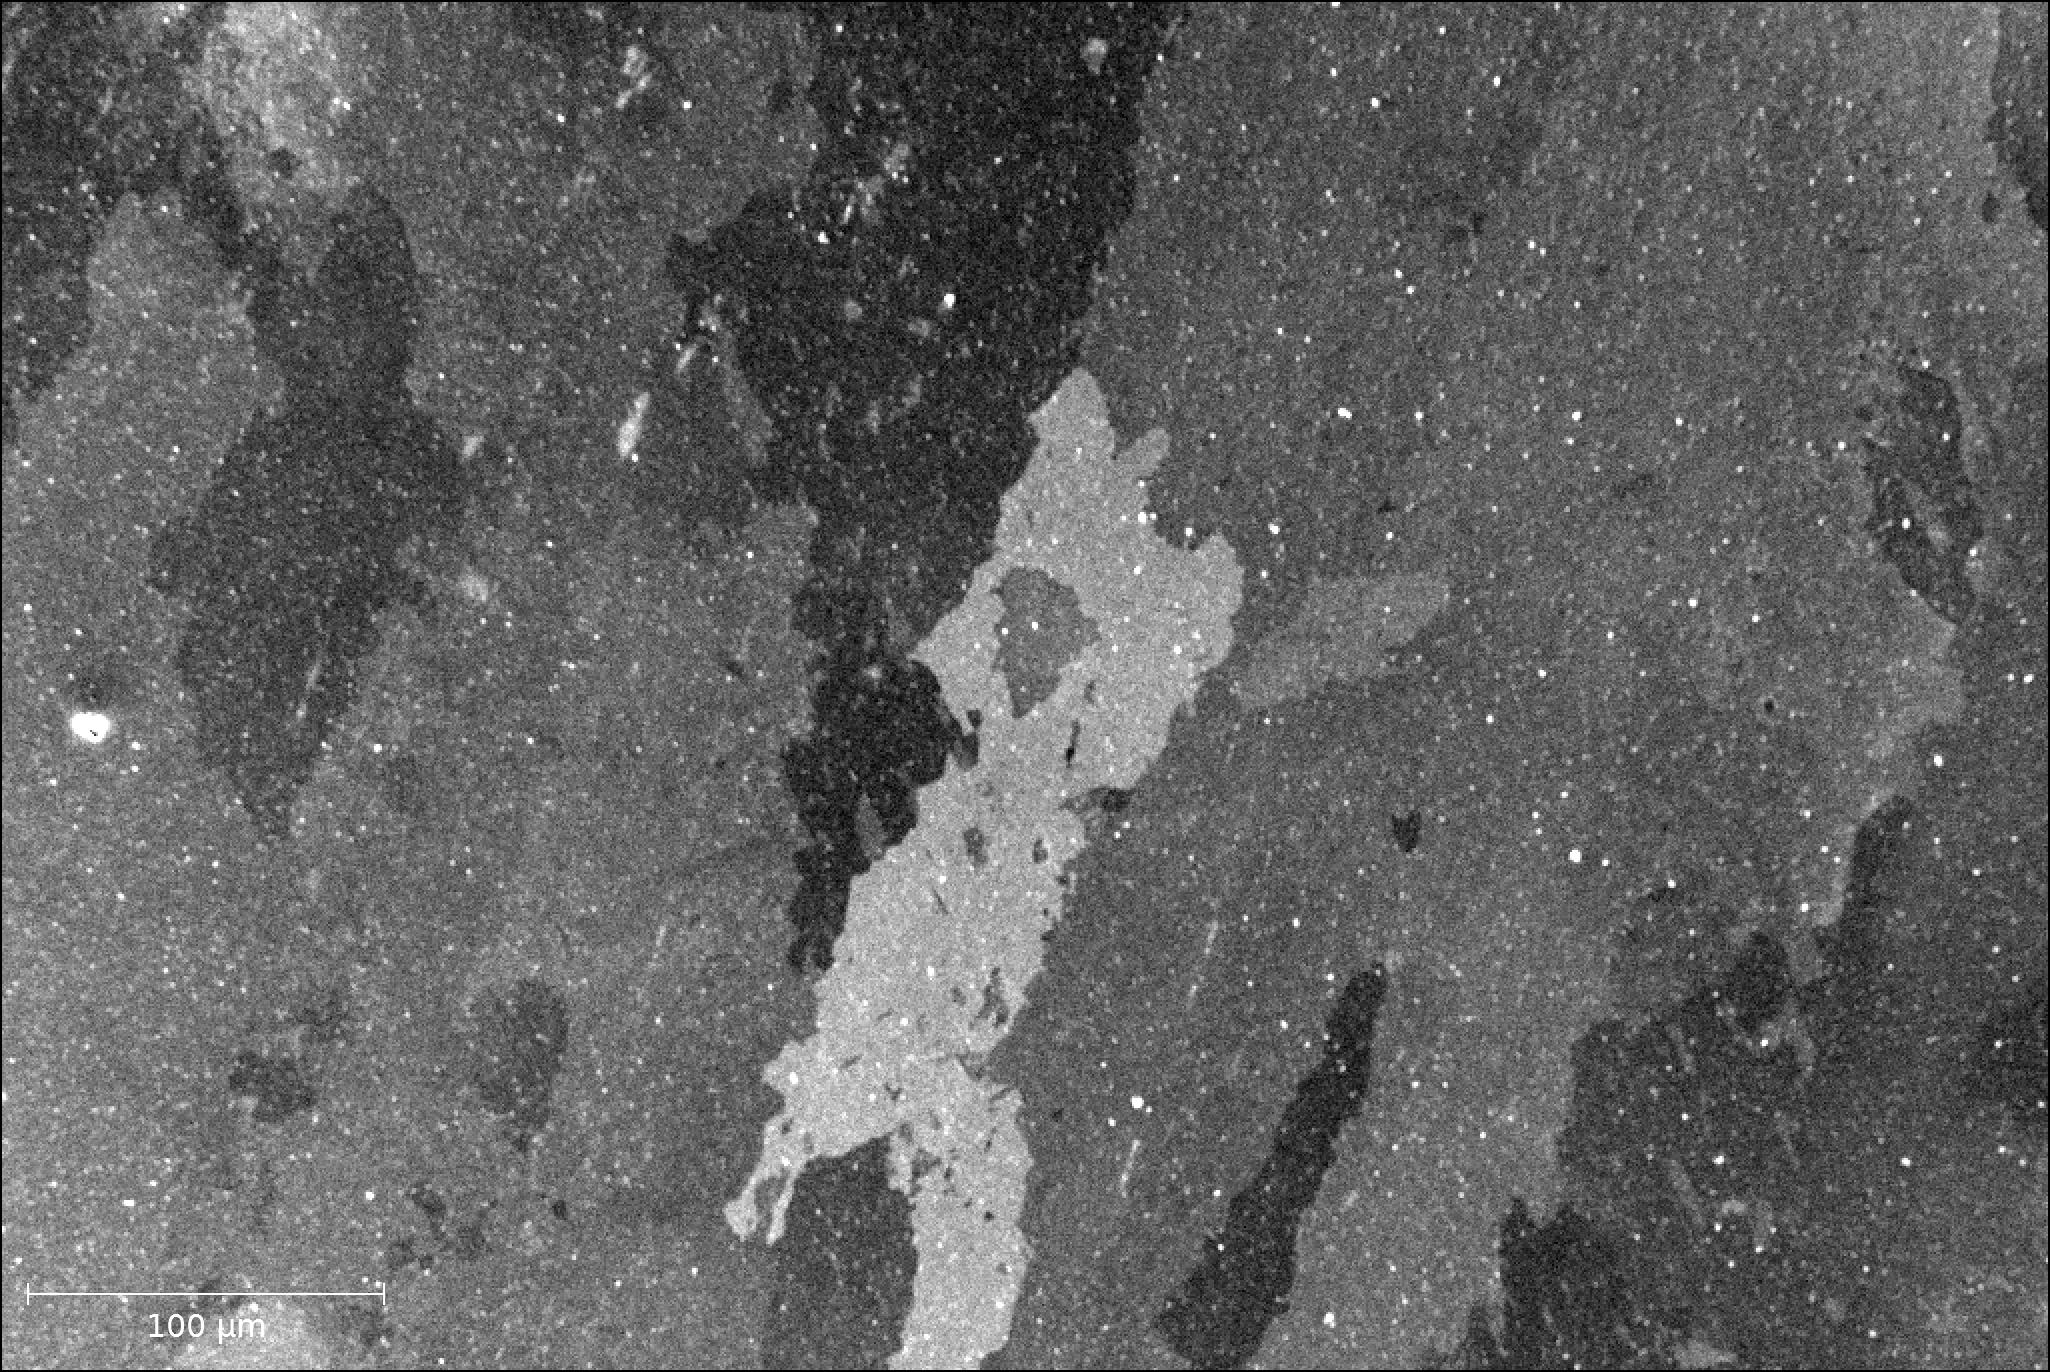
\includegraphics[width=0.45\textwidth]{./images/Domenik_16031715.jpg}
	\label{fig:SEM-1}
	
} \quad
	\subfigure[(\SI{18}{\micro \meter} x \SI{12}{\micro \meter})]{	\includegraphics[width=0.45\textwidth]{./images/Domenik_16031717.jpg}
	\label{fig:SEM-2}
}
	\caption{SEM image of etched copper foil. Different contrast suggests different grain-orientation within the surface. \subref{fig:SEM-1} Larger image showing the contrast of different grains in the copper-foil, \subref{fig:SEM-2} zoom to an area with two different contrasts and their border. \textcolor{red}{\textbf{IMAGING PARAMETERS!}}}
	\label{fig:SEM-gb}
\end{figure}

One can see in \autoref{fig:SEM-gb} that the surface imaged in different intensities which correspond to the different orientation of the copper grains within the foil\cite{wu_effects_2015}. The grain size may range from just a few \SI{}{\micro \meter} to several hundred \SI{}{\micro \meter} and in some cases even \SI{}{\milli \meter}. The grains are separated by grain boundaries. Large grains are preferred for growing graphene on copper foils because grain boundaries are subject to inhomogeneities within the graphene layer and provide a route for unwanted surface chemistry (copper oxidation for example). This effect can also be used to highlight grain boundaries as shown in \cite{wu_effects_2015}.

Although not very rough, the copper foil shows surface variation. While some areas of the sample show some wavy surface, whereas other are much flatter and appear in a different intensity (\autoref{fig:SEM-surface}).

Neither estimation on the grainsize nor guesses for their absolute orientation have been done due to the lack of EBSD-data in the SEM setup.

\begin{figure}[] \centering
		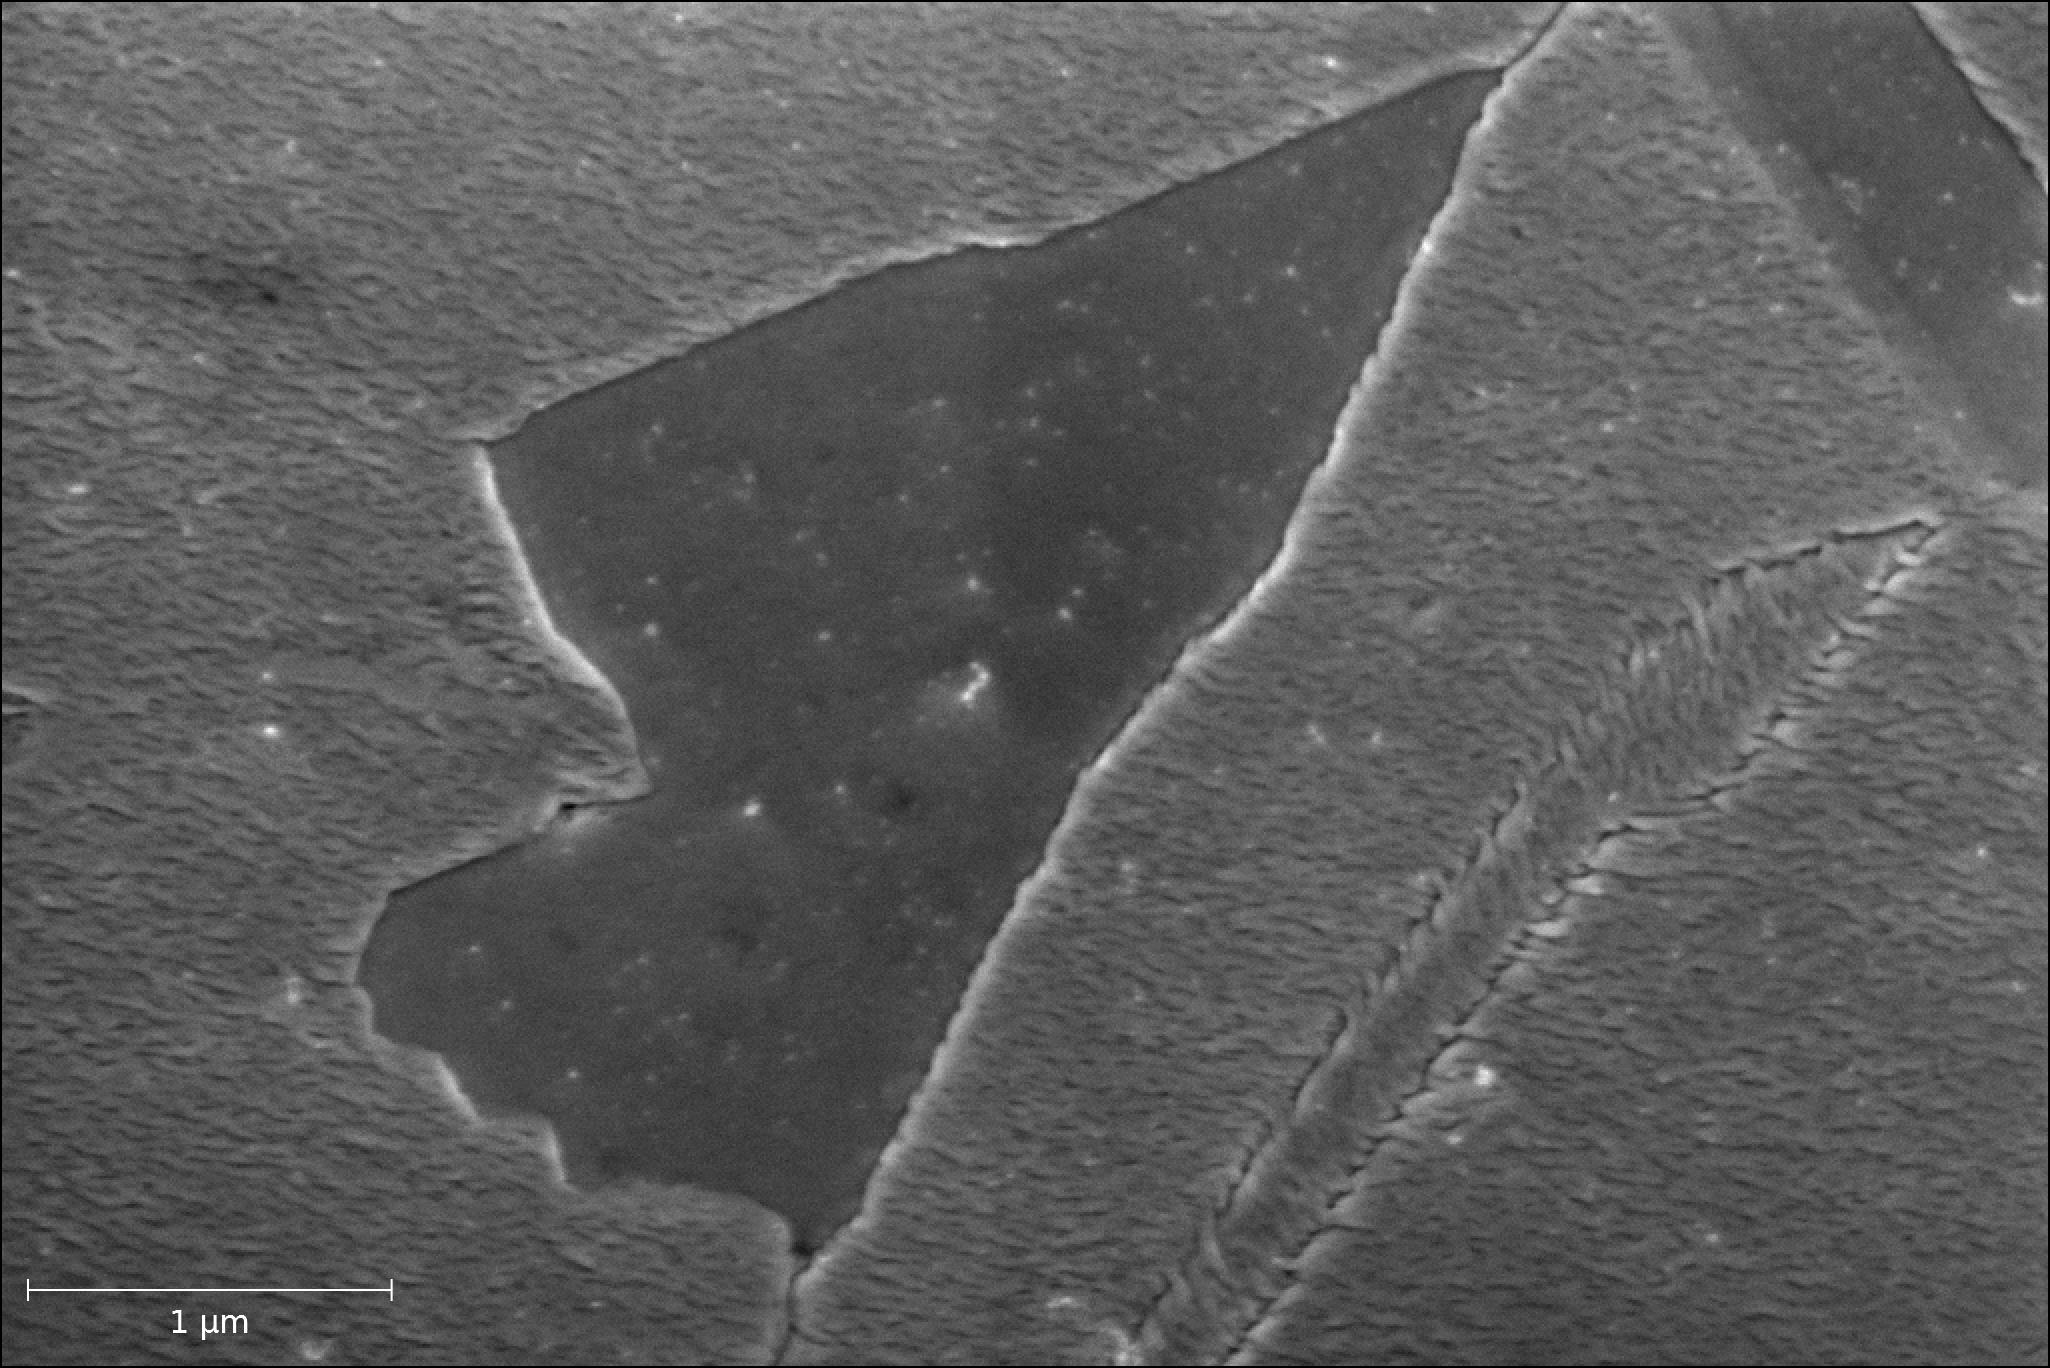
\includegraphics[width=0.7\textwidth]{./images/Domenik_16031700.jpg}
		%\includegraphics[height=6cm]{../Daten/SEM/160317-Domenik/Domenik_16031717.jpg}
	\caption{Close up SEM image that shows different surface morphologies (\SI{5.6}{\micro \meter}x\SI{3.7}{\micro \meter}). A dark grain is embedded in an otherwise curly surface. On both, bright small features are visible after etching and are attributed to an inhomogeneous etching process. \textcolor{red}{\textbf{IMAGING PARAMETERS!}}}
	\label{fig:SEM-surface}
\end{figure}



\paragraph{not done yet - maybe future?}
Some foil has been mechanically polished with 4k paper and several hours of Syton polishing. The roughness of these samples has been investigated also in AFM. These are comparable to the chemically polished ones, but are always slightly higher by $\approx 10\%$. Sometimes unwanted new scratches appear after mechanical polish.

\paragraph{STM}
\label{sec:foil-STM}
The bought and chemically polished foils are mounted on a sample holder and loaded into the load lock. It is evacuated for \SIrange{2}{3}{\hour}, afterwards the valve is opened to the chamber. During transfer, no noteable increase in the base pressure is noted. The sample is put on the parking slot.

The sample was initially degassed with slowly increasing temperatures to remove adsorbates like $CO, CO_2$ and $H_2O$.

After some time of degassing, the sample was prepared with repeated sputter and anneal cycles. The annealing temperatures were increased up to \SI{800}{\degreeCelsius}. 
After that procedure, the sample was cooled down and observed in STM.